\documentclass[aspectratio=169,xcolor={dvipsnames}]{beamer}
\usepackage[utf8]{inputenc}
\usepackage[T1]{fontenc}
\usepackage[turkish,shorthands=off]{babel}
\usepackage{lmodern}
\usepackage{graphicx}
\usepackage{amsmath}
\usepackage{amssymb}
\usepackage{booktabs}
\usepackage{textcomp} % Derece işareti gibi semboller için eklendi
\usepackage{kvsetkeys}
\let\setkeys\kvsetkeys
\usepackage{rotating}
\usepackage{xcolor}
\usepackage{tikz}
\usepackage{listings}
\usepackage{transparent}
\usepackage{hyperref}
\shorthandoff{=!:}
\AtBeginDocument{\shorthandoff{=!:}}
% Tema seçimi
\usetheme{Madrid}
\usecolortheme{seahorse}

% Logo overlay komutu (her slaytta tekrar etmek yerine)
\newcommand{\bglogo}{%
\begin{tikzpicture}[remember picture, overlay]
    \node at (current page.center)
      {{\transparent{0.18}
        
\includegraphics[width=0.8\paperwidth]{images/logo.png}
      }};
\end{tikzpicture}%
}

% Eklenen süreç görselleri dosya olarak mevcutsa kullanılır; yoksa derleme bozulmaz.
\newcommand{\processvisual}[3]{%
\IfFileExists{#1}{%
\begin{center}
\includegraphics[width=\paperwidth,height=0.82\paperheight,keepaspectratio]{#1}
\end{center}
}{%
\bglogo
\begin{block}{#2}
#3
\end{block}
\begin{alertblock}{Görsel dosyası bekleniyor}
\texttt{\detokenize{#1}} dosyasını \texttt{images} klasörüne eklediğinizde bu slaytta otomatik olarak ilgili görsel kullanılacaktır.
\end{alertblock}
}%
}

\newcommand{\processvisualwithfallback}[4]{%
\IfFileExists{#1}{%
\begin{center}
\includegraphics[width=\paperwidth,height=0.82\paperheight,keepaspectratio]{#1}
\end{center}
}{%
\begin{center}
\includegraphics[width=\paperwidth,height=0.68\paperheight,keepaspectratio]{#4}
\end{center}
\vspace{-0.2cm}
\begin{alertblock}{Yeni görsel dosyası bekleniyor}
\small \texttt{\detokenize{#1}} dosyasını \texttt{images} klasörüne eklediğinizde bu slaytta eski diyagram yerine yeni görsel kullanılacaktır.
\end{alertblock}
}%
}

\newcommand{\facilityphoto}[4][]{%
\IfFileExists{#2}{%
\centering
\includegraphics[width=\linewidth,height=#3,keepaspectratio,#1]{#2}
}{%
\begin{center}
\fbox{%
\begin{minipage}[c][#3][c]{0.92\linewidth}
\centering
\textbf{#4}\\[0.2cm]
\small Fotoğraf dosyası bekleniyor:\\
\texttt{\detokenize{#2}}
\end{minipage}}
\end{center}
}%
}

% Başlık bilgileri
\title[Proje No: 190871]{\textbf{QuatMark-EQCore}: Dijital İçerik Sahteciliğine Karşı Eliptik Kuaterniyon ve Kaotik Kriptografi Tabanlı Dayanıklı Damgalama Çekirdeğinin Geliştirilmesi}
\subtitle{\texorpdfstring{
\includegraphics[height=2.9ex]{images/pngegg.png} }{}TÜBİTAK 1507 -- KOBİ Ar-Ge Başlangıç Destek Programı}
\author{\textcolor{Turquoise}{\textbf{QuatVision Yazılım Teknoloji San. Tic. A.Ş.}}}
%\institute{Proje No: 190871 / Başvuru No: 7260583}

\begin{document}

% Başlık sayfası
\begin{frame}
\titlepage
\end{frame}

% İçindekiler
\begin{frame}{İçindekiler}
\bglogo
\tableofcontents
\end{frame}

% =====================================================================
% Bölüm 1: Proje Tanıtımı
% =====================================================================
\section{Proje Tanıtımı}

\begin{frame}{Proje Özeti}
\bglogo
\begin{block}{Proje Adı}
\textbf{QuatMark-EQCore}: Dijital İçerik Sahteciliğine Karşı Eliptik Kuaterniyon ve Kaotik Kriptografi Tabanlı Dayanıklı Damgalama Çekirdeğinin Geliştirilmesi
\end{block}

\begin{itemize}
\item \textbf{Proje Numarası:} 190871 \hspace{0.4cm} \textbf{Başvuru No:} 7260583
\item \textbf{Kuruluş:} QuatVision Yazılım Teknoloji San. Tic. A.Ş.
\item \textbf{Program:} TÜBİTAK 1507 -- KOBİ Ar-Ge Başlangıç Destek Programı
\item \textbf{Proje Süresi:} 16 ay (01.06.2026 -- 30.09.2027)
\item \textbf{Teknoloji Grubu:} Bilişim Teknolojileri
\item \textbf{THS Başlangıç:} 3 $\rightarrow$ \textbf{THS Hedef:} 8
\item \textbf{Toplam Bütçe:} $\sim$1.841.233 TL \hspace{0.3cm} \textbf{Toplam Adam-Ay:} 30,72
\end{itemize}
\end{frame}

\begin{frame}{Kuruluş Tanıtımı}
\bglogo
\begin{block}{QuatVision Hakkında}
QuatVision; bilgisayar görüsü, dijital veri güvenliği ve dijital damgalama alanlarında faaliyet gösteren, Eylül 2025'te kurulmuş Ar-Ge odaklı bir teknoloji girişimidir.
\end{block}

\textbf{Öz Yetkinlikler:}
\begin{itemize}
\item Yüksek matematik 
\item Görüntü işleme ve derin öğrenme algoritmaları
\item Veri güvenliği ve dijital damgalama teknolojileri
\item Yapay zekâ tabanlı görsel denetim sistemleri
\end{itemize}

\textbf{Vizyon:} Dijital içeriklerin güvenliği, kimlik doğrulaması ve izlenebilirliği konusunda ulusal ve uluslararası ölçekte öncü bir teknoloji şirketi olmak.
\end{frame}

\begin{frame}{Kuruluş Altyapısı}
\bglogo
\begin{block}{Fiziksel Konum ve Ar-Ge Ortamı}
QuatVision, \textbf{Sakarya Teknokent} çatısı altında kurulmuş, Ar-Ge ve teknoloji geliştirme ekosistemi içinde konumlanan bir şirkettir. Şirketin proje yürütümü için kullandığı \textbf{45 m$^2$ ofis alanı}; yazılım geliştirme, algoritma tasarımı, test/analiz çalışmaları ve proje koordinasyonu için yeterli çalışma ortamı sunmaktadır.
\end{block}


\textbf{Konum Avantajı}
\begin{itemize}
\item Teknokent ekosistemi içinde Ar-Ge odaklı çalışma ortamı
\item Üniversite-sanayi etkileşimine ve akademik danışmanlık süreçlerine yakınlık
\item Proje toplantıları, dokümantasyon ve yazılım geliştirme için uygun ofis düzeni
\end{itemize}


\end{frame}

\begin{frame}{Sakarya Teknokent ve Ofis Altyapısı}
\bglogo
\begin{columns}
\column{0.5\textwidth}
\begin{block}{\makebox[\linewidth][c]{Sakarya Teknokent Binası}}
\facilityphoto[trim=0 430 0 436,clip]{images/bina.jpeg}{4.5cm}{Sakarya Teknokent Binası}
\end{block}

\column{0.5\textwidth}
\begin{block}{\makebox[\linewidth][c]{QuatVision Ofisi}}
\facilityphoto{images/ofis.jpeg}{4.5cm}{QuatVision Ofisi}
\end{block}
\end{columns}


\end{frame}

\begin{frame}{Mevcut Kurumsal ve Teknik Hazırlık}
\bglogo
\begin{block}{Mevcut Ürün Altyapısı}
\begin{itemize}
\item QuatMark SaaS platformu halihazırda geliştirilmiştir.
\item RESTful API ve ödeme altyapısı öz kaynaklarla oluşturulmuştur.
\item Mevcut QuatMark ürünümüz, QR ayrışımı tabanlı kör renkli görüntü damgalama çekirdeği ile \textcolor{MidnightBlue}{\textbf{telif hakkı koruması}}, \textcolor{MidnightBlue}{\textbf{kimlik doğrulama}}, \textcolor{MidnightBlue}{\textbf{sızıntı önleme}} ve \textcolor{MidnightBlue}{\textbf{yayın izleme}} hizmetlerini yerine getirmektedir.
\item Yeni proje, bu ürünün damgalama çekirdeğini yenilemeyi hedefler.
\end{itemize}
\end{block}

\vfill
{\scriptsize \textbf{Referans:} Q. Su, Y. Niu, G. Wang, S. Jia ve J. Yue, ``Color image blind watermarking scheme based on QR decomposition'', \textit{Signal Processing}, 94 (2014), 219--235.}
\end{frame}

\begin{frame}{Mevcut QuatMark Ürünü ve Yeni Çekirdek İhtiyacı}
\bglogo
\begin{block}{Mevcut Durum}
QuatMark ürünü; SaaS platformu, RESTful API ve ödeme altyapısı bileşenleriyle birlikte şirketimizin \textbf{öz kaynaklarıyla geliştirilmiştir} .
\end{block}

\begin{alertblock}{Mevcut Çekirdeğin Dezavantajları}
\begin{itemize}
\item Renk korelasyonu kaybı (RGB kanalları ayrı işleniyor)
\item Damga yerleştirme asenkronizasyonu
\item İki katmanlı güvenlik yapısı(MD5+Arnold)
\item Geometrik ve Derin öğrenme tabanlı saldırılara karşı sınırlı dayanıklılık
\end{itemize}
\end{alertblock}

\textbf{Yeni Proje Odağı:} Mevcut ürünün damgalama \textbf{çekirdeğindeki} bu dezavantajları gideren, günümüzün dijital güvenlik tehditlerine cevap veren yeni nesil çekirdek (\textbf{QuatMark-EQCore}) geliştirmek.
\end{frame}

% =====================================================================
% Bölüm 2: Projenin Amacı
% =====================================================================
\section{Projenin Amacı ve Hedefleri}

\begin{frame}{Bilgi Güvenliği}
\bglogo
\begin{block}{Tanım}
Dijital teknolojilerin hızla gelişmesiyle birlikte, internet üzerinden paylaşılan verilerin güvenliği giderek daha önemli hâle gelmiştir. \textcolor{red}{Özellikle kişisel verilerin korunması, fikri mülkiyet haklarının güvenliği ve dijital içeriklere yönelik sahteciliğe karşı alınacak önlemler günümüzde büyük bir öncelik taşımaktadır.} \textbf{Bu bağlamda, bilgi güvenliği teknolojileri, dijital verilerin bütünlüğünü ve gizliliğini sağlamada kritik bir rol oynamaktadır.}
\end{block}

\begin{figure}[h]
    \centering
    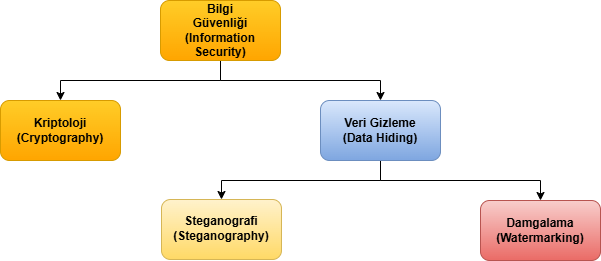
\includegraphics[scale=0.35]{images/data_hiding.png}
\end{figure}
\end{frame}

%\begin{frame}{Bilgi Güvenliği: Kriptoloji ve Veri Gizleme}
%\bglogo
%\begin{block}{Kriptoloji}
%Verilerin şifrelenmesi ve kodlanması yoluyla, yalnızca yetkili erişimin sağlanması amacıyla kullanılan yöntemleri içerir.
%\end{block}
%\begin{block}{Veri Gizleme}
%Verinin yapısına veya taşıyıcı medyaya entegre edilen ek bilgilerin, yalnızca yetkili kullanıcılar tarafından tespit edilip okunabilmesini sağlayacak biçimde saklanması süreci olarak tanımlanır.
%\end{block}

%\textcolor{red}{Veri gizleme işlemi, kriptoloji yöntemleriyle de gerçekleştirilebilir. Ancak gizlenecek verinin şifrelenmiş ve erişilebilir olması, saldırganların ilgisini artırmakta ve güvenlik açısından ek riskler doğurmaktadır.}
%\end{frame}

\begin{frame}{Watermarking (Dijital Damgalama) Nedir?}
\bglogo
\begin{block}{Tanım}
Dijital damgalama (watermarking), bir dijital veriye (görüntü, ses, video, metin) gözle görülür veya görünmez bir bilgi (imza, logo, kimlik kodu) ekleme işlemidir.
\end{block}

\begin{figure}[h]
    \centering
    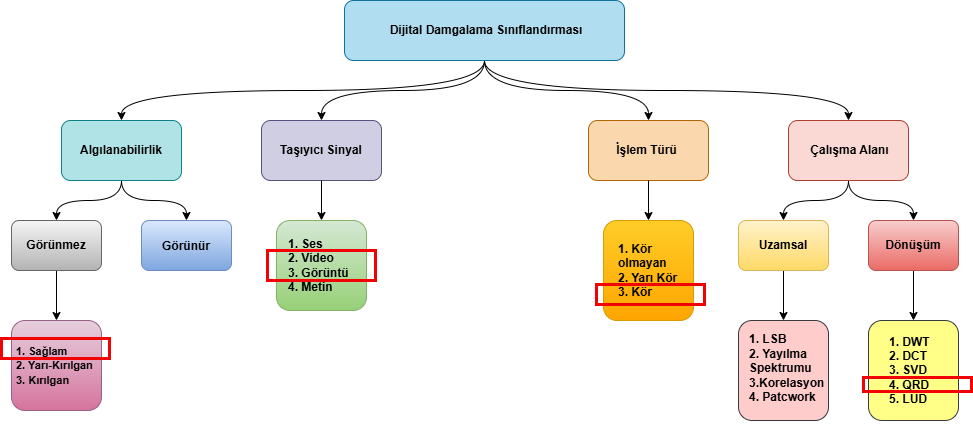
\includegraphics[scale=0.33]{images/siniflandirma.png}
\end{figure}
\end{frame}

\begin{frame}{Neden Günümüzde İhtiyaç Duyuluyor?}
\bglogo
\begin{alertblock}{Artan Dijital Tehditler}
Yapay zekâ tabanlı içerik üretim araçları (deepfake, generative AI) ile dijital içeriklerin kopyalanması, manipüle edilmesi ve izinsiz dağıtılması her zamankinden daha kolay hâle gelmiştir.
\end{alertblock}

\textbf{Karşılaşılan Temel Sorunlar:}
\begin{itemize}
\item \textbf{Dijital Sahtecilik (Deepfake):} Yapay zekâ ile üretilen sahte içerikler (video, ses, görüntü) güveni sarsmaktadır.
\item \textbf{Veri Sızıntıları:} Kurumsal/askeri gizli belgelerin kim tarafından sızdırıldığını bilme ihtiyacı artmıştır.
\item \textbf{Telif Hakkı İhlalleri:} Fotoğraf, video ve dijital sanat eserlerinin izinsiz kopyalanması içerik üreticilerini mağdur etmektedir.
\item \textbf{Bütünlük Kaybı:} Bir medyanın (adli delil, tıbbi görüntü) orijinalliğini kanıtlama zorunluluğu vardır.
\end{itemize}
\end{frame}

\begin{frame}{AB Yapay Zekâ Yasası: Madde 50}
\bglogo
\begin{alertblock}{Regülasyonun Getirdiği Yeni Zorunluluk}
AB Yapay Zekâ Yasası'nın 50. maddesi kapsamında, sentetik \textbf{ses, görsel, video ve metin} üreten yapay zekâ sistemlerinin çıktılarının \textbf{makine tarafından okunabilir} biçimde işaretlenmesi ve yapay/manipüle edilmiş olduğunun tespit edilebilir olması beklenmektedir.
\end{alertblock}

\textbf{Teknik beklenti:}
\begin{itemize}
\item Dijital varlık üzerinde otomatik okunabilir işaretleme/damgalama
\item Görünür etiketten bağımsız, \textbf{silinmeye ve manipülasyona dayanıklı} doğrulama izi
\item Etkili, birlikte çalışabilir, sağlam ve güvenilir tespit mekanizması
\item Farklı içerik türlerinde çalışabilen standart uyumlu altyapı
\end{itemize}

\vspace{0.1cm}
{\scriptsize Kaynak: Regulation (EU) 2024/1689, Article 50. Şeffaflık yükümlülükleri 2 Ağustos 2026 itibarıyla uygulanmaya başlayacaktır.}
\end{frame}

\begin{frame}{C2PA: Küresel İçerik Kimlik Standardı}
\bglogo
\begin{block}{Coalition for Content Provenance and Authenticity}
C2PA, dijital içeriğin \textbf{kaynağını, üretim geçmişini, düzenlemelerini ve yapay zekâ kullanım bilgisini} doğrulanabilir biçimde taşımak için geliştirilen açık bir teknik standarttır.
\end{block}

\begin{columns}
\column{0.52\textwidth}
\textbf{Content Credentials yaklaşımı:}
\begin{itemize}
\item Kriptografik olarak bağlı içerik kimliği
\item Kaynak, işlem geçmişi ve değişiklik kayıtları
\item Görsel, video, ses ve belge ekosistemine uyum
\end{itemize}

\column{0.48\textwidth}
\begin{alertblock}{EQCore ile Tamamlayıcı Değer}
C2PA içeriğin \textbf{kimliğini ve geçmişini} taşırken, EQCore içeriğin içine \textbf{dayanıklı ve görünmez damga} yerleştirerek doğrulama izini güçlendirir.
\end{alertblock}
\end{columns}

\vspace{0.1cm}
{\scriptsize Kaynak: C2PA resmi teknik standardı ve C2PA Conformance Programme.}
\end{frame}

\begin{frame}{Türkiye İçin İlk Olma Fırsatı}
\bglogo
\small
\begin{alertblock}{Stratejik Pazar Boşluğu}
Türkiye'de, AB YZ Yasası Madde 50 uyum ihtiyacına yönelik \textbf{yerli, patentli, C2PA uyumluluğunu hedefleyen ve uçtan uca dijital damgalama/doğrulama hizmeti} sunan bir şirket bulunmadığı değerlendirilmektedir.
\end{alertblock}

\textbf{QuatMark-EQCore hedefi:}
\begin{itemize}
\item Yerli ve milli, patent korumalı dayanıklı damgalama çekirdeği
\item C2PA sertifikasyonu/uyumluluğu ile küresel standartlara entegrasyon
\item Görsel, ses, video ve metin varlıkları için SaaS/API tabanlı doğrulama
\item Türkiye'de sektörün öncü ürünü, Avrupa regülasyonlarına uyumlu ihracat potansiyeli
\end{itemize}

\begin{block}{Projenin Güçlü Konumlanması}
Regülasyon baskısı, C2PA standardizasyonu ve yerli çözüm eksikliği aynı anda oluştuğu için QuatMark-EQCore \textbf{erken girilecek stratejik bir uyum pazarı} fırsatıdır.
\end{block}
\end{frame}

\begin{frame}{Kullanım Alanları ve Pazar Potansiyeli}
\bglogo
\begin{columns}
\column{0.55\textwidth}
\begin{block}{Yaygın Kullanım Alanları}
\tiny
\begin{itemize}
\item \textbf{Askeri Uygulamalar:} Gizli belge ve stratejik veri korunumu.
\item \textbf{Telif Hakkı Koruma:} İçerik sahipliği, izinsiz kopyalama engeli.
\item \textbf{Dijital Adli Tıp:} Manipülasyon izlerinin doğrulanması.
\item \textbf{Uzaktan Eğitim:} Ders materyali / sınav bütünlüğü.
\item \textbf{Akıllı Sağlık:} Hasta verisi gizliliği, sahtecilik önleme.
\item \textbf{Güvenli E-Oylama:} Oy pusulası doğrulama.
\item \textbf{Lisans Güvenliği:} Yazılım/medya korsanlığını önleme.
\item \textbf{Yayın İzleme:} Platformlar arası içerik takibi.
\end{itemize}
\end{block}
\column{0.45\textwidth}
\begin{alertblock}{Pazar Potansiyeli (Grand View Research)}
\scriptsize
YZ Yasası, C2PA ve deepfake riskleri pazarın özellikle \textbf{AI watermarking} tarafında hızlanmasına yol açmaktadır.
\vspace{0.15cm}

\textbf{Genel Dijital Damgalama:}
\begin{itemize}
\item 2024: 1.45 Milyar USD
\item 2033: 3.80 Milyar USD
\item CAGR: \%11.4
\end{itemize}

\textbf{AI Watermarking Segmenti:}
\begin{itemize}
\item 2024: 427.2 Milyon USD
\item 2033: \textbf{3.07 Milyar USD}
\item CAGR: \textbf{\%25.3}
\end{itemize}
\end{alertblock}
\end{columns}
\end{frame}

\begin{frame}{Çözülmesi Amaçlanan Problem}
\bglogo
\begin{alertblock}{Mevcut Damgalama Teknolojilerinin Yapısal Zafiyetleri}
\begin{itemize}
\item \textbf{Renk Korelasyonu Kaybı:} RGB kanalları bağımsız işlendiğinden kanallar arası matematiksel ilişki yok olmakta, görsel kalite kayıpları doğmaktadır.
\item \textbf{Damga Asenkronizasyonu:} Her kanalın bağımsız işlenmesi, damganın eş zamanlı tutarlı yerleşmesini engellemekte, dayanıklılığı zayıflatmaktadır.
\item \textbf{Kapalı Yabancı Çözümler:} Digimarc, Imatag, Verimatrix/Irdeto, MarkAny, Google SynthID -- temel algoritmalar ticari sır kapsamında, yerli alternatif yok.
\item \textbf{Derin Öğrenme Saldırıları:} Denoiser/autoencoder/difüzyon modelleri klasik damgaları silebilmektedir; rakip ürünlerde \textbf{kamuya açık savunma yok.}
\end{itemize}
\end{alertblock}
\end{frame}

\begin{frame}{Projenin Temel Amacı}
\bglogo
\begin{alertblock}{Ana Hedef}
Mevcut QuatMark ürününün damgalama altyapısını yenilemek üzere, eliptik kuaterniyon QR ayrışımı ve kaotik kriptografi katmanını bir araya getiren özgün \textbf{QuatMark-EQCore} çekirdeğini geliştirmek.
\end{alertblock}

\textbf{Çekirdeğin Üç Somut Bileşeni:}
\begin{enumerate}
\item Eliptik kuaterniyon uzayında \textbf{Householder dönüşümü ve QR ayrışımı teorisi}
\item Çok katmanlı güvenlik mimarisine sahip \textbf{damgalama modeli}
\item Çekirdeğin mevcut QuatMark ürününe \textbf{entegrasyonu ve pilot doğrulama}
\end{enumerate}

\textbf{Hizmet Çıktıları:}
\begin{itemize}
\item[1.] Veri Sızıntılarını Önleme ve Tespit
\item[2.] İçerik ve Kimlik Doğrulama
\item[3.] Fikri Mülkiyet Haklarını Koruma
\end{itemize}
\end{frame}

\begin{frame}{Hizmet 1: Veri Sızıntılarını Önleme ve Tespit}
\bglogo
\begin{block}{Sızıntı Tespit Senaryosu}
Hassas bir belge veya askeri bir görsel birden fazla departmanla/kişiyle paylaşıldığında belgenin güvenliği için:
\end{block}
\textbf{QuatMark-EQCore Çözümü:}
\begin{itemize}
\item Her bir kopyaya, alıcıya özel, görünmez bir \textbf{dijital parmak izi} eklenir.
\item İçerik yetkisiz bir yerde yayınlanırsa, sızan belgedeki damga okunur.
\item Sızıntının \textbf{hangi kullanıcıdan} kaynaklandığı tespit edilir.
\item İçeriden gelen tehditlere karşı en güçlü caydırıcılığı sağlar.
\end{itemize}
\end{frame}

\begin{frame}{Sızıntı Tespiti ve Kaynak İzleme Süreci}
\processvisual{images/sizinti_tespiti_sureci.png}{Sızıntı Tespiti ve Kaynak İzleme}
{Alıcıya özel görünmez damga ile kişiselleştirme, güvenli dağıtım, sızan içerikten damga çözümleme ve kaynak raporlama akışı gösterilir.}
\end{frame}

\begin{frame}{Hizmet 2: İçerik Kimlik Doğrulama (Bütünlük)}
\bglogo
\begin{block}{Kimlik Doğrulama}
Özellikle yapay zekâ (Deepfake) çağında, bir görüntünün veya belgenin orijinal mi yoksa tahrif edilmiş mi olduğunu anlamak kritiktir.
\end{block}
\textbf{QuatMark-EQCore Çözümü:}
\begin{itemize}
\item Orijinal içeriğe gömülen damga, bir \textbf{dijital mühür} görevi görür.
\item \textbf{Doğrulama:} Damga okunabiliyorsa içerik \textbf{orijinaldir} ve değiştirilmemiştir.
\item Adli bilişim, tıbbi görüntüler ve haber ajansları için hayati önem taşır.
\end{itemize}
\end{frame}

\begin{frame}{İçerik Doğrulama ve Bütünlük Kontrol Süreci}
\processvisual{images/icerik_dogrulama_sureci.png}{İçerik Doğrulama ve Bütünlük Kontrol}
{Orijinal içeriğe bütünlük damgası gömme, şüpheli içeriği sorgulama, damga varlığı ve değişiklik analizi ile ayrıntılı bütünlük raporu üretme akışı özetlenir.}
\end{frame}

\begin{frame}{Kimlik Doğrulama ve Sahiplik Teyit Süreci}
\processvisual{images/kimlik_dogrulama_sureci.png}{Kimlik Doğrulama ve Sahiplik Teyidi}
{İçeriğe sahiplik bilgisinin görünmez damga olarak işlenmesi, doğrulama talebi, damga okuma, kimlik eşleştirme ve raporlama adımları gösterilir.}
\end{frame}

\begin{frame}{Hizmet 3: Fikri Mülkiyet Haklarını Koruma}
\bglogo
\begin{block}{Telif Hakkı}
Bir fotoğrafçı, dijital sanatçı veya içerik üreticisi, eserlerinin internette izinsiz kopyalanmasından ve "çalıntı" olarak kullanılmasından endişe duymaktadır.
\end{block}
\textbf{QuatMark-EQCore Çözümü:}
\begin{itemize}
\item Eserin içine, sahibinin kimlik bilgilerini içeren görünmez bir damga yerleştirilir.
\item Eser internette izinsiz kullanılırsa, damga çıkarılarak eserin \textbf{gerçek sahibi} kanıtlanabilir.
\item Dijital korsanlığa karşı caydırıcılık sağlar.
\item Olası telif hakkı davalarında \textbf{güçlü yasal kanıt} niteliği taşır.
\end{itemize}
\end{frame}

\begin{frame}{Telif Hakkı Koruma ve Sahiplik Kanıtlama Süreci}
\processvisual{images/telif_hakki_sureci.png}{Telif Hakkı Koruma ve Sahiplik Kanıtlama}
{Dijital içeriğe telif damgası gömme, platform taraması, damga eşleştirme, sahiplik doğrulama ve hukuki kanıt raporu üretme süreci açıklanır.}
\end{frame}

\begin{frame}{Somut ve Ölçülebilir Başarı Ölçütleri}
\bglogo
\begin{table}
\centering
\small
\begin{tabular}{p{6cm}p{6cm}}
\toprule
\textbf{Başarı Ölçütü} & \textbf{Hedeflenen Değer} \\
\midrule
Eliptik kuaterniyon QR ayrışımı (4$\times$4) & Hız $<$ 0,184 ms \\
QR ayrışımı yeniden yapılandırma hatası & $\leq$ 1e-16 \\
Görüntü kalitesi (PSNR) & $>$ 40 dB \\
Yapısal benzerlik (SSIM) & $>$ 0,98 \\
Saldırısız çıkarma korelasyonu (NC) & $=$ 1 \\
Geleneksel saldırılarda dayanıklılık (NC) & $\geq$ 0,98 \\
Derin öğrenme saldırılarında dayanıklılık (NC) & $\geq$ 0,95 \\
\bottomrule
\end{tabular}
\end{table}
\end{frame}

% =====================================================================
% Bölüm 3: Yenilikçi Yönler ve Teknik Altyapı
% =====================================================================
\section{Yenilikçi Yönler ve Teknik Altyapı}

% \begin{frame}{Görünmez Damgalama}
% \bglogo
% \begin{block}{Görünmez Damgalama}
% Bu yöntemler, yasal delil niteliği sunma ve manipülasyona karşı yüksek dayanıklılık gibi avantajlara sahiptir.
% \end{block}

% \begin{block}{Temel Dezavantajlar}
% \begin{itemize}
% \item \textbf{Yüksek Hesaplama Gereksinimi:} Görünmezlik ile dayanıklılığı (robustness) bir arada sağlamak için karmaşık algoritmalar yoğun işlem gücü gerektirir.
% \item \textbf{Güvenli Anahtar Yönetimi:} Algoritma güvenliği, gömme/çıkarma anahtarlarının gizliliğine ve yönetimine bağlıdır.
% \end{itemize}
% \end{block}
% \end{frame}

% \begin{frame}{Kör Damgalama}
% \bglogo
% \begin{block}{Kör Damgalama}
% Ana dosyanın saklanmasının veya iletilmesinin zor olduğu durumlarda avantaj sağlar; medya dağıtımı, film, müzik, dijital yayınlarda ana veriye erişmeden damga doğrulama imkânı sunar.
% \end{block}

% \begin{itemize}
% \item \textbf{Doğruluk ve Kesinlik Problemleri:} Ana referans olmadığından damga çıkarımında doğruluk sorunları doğabilir.
% \item \textbf{Dayanıklılık Zafiyetleri:} Bazı durumlarda saldırılara karşı direnç zayıflayabilir.
% \item \textbf{Kalite Kaybı Riski:} Görüntü işleme operasyonları (sıkıştırma vb.) damgaya zarar verebilir.
% \end{itemize}
% \end{frame}

% \begin{frame}{Dönüşüm Uzayı Yöntemleri}
% \bglogo
% \begin{block}{Dönüşüm Uzayı}
% Saldırılara karşı daha güçlü direnç ve damga bilgisinin görüntü kalitesini büyük ölçüde koruyacak şekilde saklanabilmesi gibi avantajlara sahiptir.
% \end{block}
% \begin{block}{Dezavantajlar}
% \begin{itemize}
% \item Yüksek hesaplama maliyeti
% \item Düşük gömme kapasitesi
% \end{itemize}
% \end{block}
% \begin{block}{Kalite Bozulması Riski}
% Dönüştürülmüş bileşenlerin yanlış seçimi ya da uygunsuz güç parametreleri, görüntü kalitesinde gözle görülür bozulmalara neden olabilir.
% \end{block}
% \end{frame}

\begin{frame}{Renkli Görüntü Damgalama Modelleri}
\bglogo
\begin{block}{Geleneksel Yaklaşım: Kanalların Ayrı İncelenmesi}
Hem ana görüntünün hem de damga görüntüsünün renk kanallarının (R, G, B) ayrı ayrı incelenmesi neticesinde:
\begin{itemize}
\item Renk kanallarının \textbf{korelasyon kaybı}
\item Damga yerleştirmenin \textbf{asenkronizasyonu}
\end{itemize}
gibi dezavantajlar ortaya çıkmaktadır.
\end{block}

\begin{alertblock}{Bu Durumun Sonuçları}
\begin{itemize}
\item Modelin doğruluğunun ve verimliliğinin azalması
\item İşleme süresinin artması, sonuçların tutarsız olması
\end{itemize}
\end{alertblock}
\end{frame}

% \begin{frame}{Reel Kuaterniyonlar: Zorluklar}
% \bglogo
% \begin{block}{Avantaj}
% Reel kuaterniyonlar, çok kanallı verilerin senkron işlenmesinde güçlü bir araçtır; daha az parametreyle daha zengin ilişkiler modelleyebilir.
% \end{block}
% \begin{alertblock}{Dezavantaj: Çarpma İşleminin Değişmeli Olmaması}
% \begin{itemize}
% \item Ek hesaplama maliyeti
% \item Algoritmik karmaşıklık
% \item Hata birikimi (yeniden sıralama yapılamaz)
% \end{itemize}
% \end{alertblock}
% \begin{block}{Cebirsel Yapının Benzersiz Olmaması}
% \begin{itemize}
% \item \textbf{Bölme:} Soldan/sağdan iki tanım
% \item \textbf{Özdeğer:} Sol/sağ özdeğer çift anlamlılığı
% \end{itemize}
% $\Rightarrow$ Denklem çözmede ve damga çıkarmada \textbf{belirsizlik}, modelde \textbf{karmaşıklık} artışı.
% \end{block}
% \end{frame}

\begin{frame}{Projenin Yenilikçi Yönleri}
\bglogo
\begin{block}{Temel Yenilik}
4-boyutlu \textbf{eliptik kuaterniyonlar} uzayı üzerine inşa edilen, \textbf{değişmeli (komütatif)} cebir yapısına sahip damgalama çekirdeği.
\end{block}

\textbf{Üç Eksende Özgünlük:}
\begin{enumerate}
\item \textbf{Akademik:} Householder dönüşümü ve QR ayrışımı eliptik kuaterniyon uzayında \textit{literatürde ilk kez} formüle edilecek.
\item \textbf{Güvenlik:} Arnold karıştırma + kaotik kriptografi + p-hiperparametresi + \textbf{SHA-2} tabanlı pseudo-rastgele konum seçimi $\rightarrow$ \textbf{çok katmanlı} mimari.
\item \textbf{Performans:} Değişmeli cebir yapısı $\rightarrow$ daha düşük algoritmik karmaşıklık, uç nokta cihazlarda çalışabilme potansiyeli.
\end{enumerate}

\textbf{Teknik Avantajlar:} RGB bütünleşik işleme, korelasyon kaybı yok, senkronizasyon hatası yok, yüksek performans (4$\times$4 QR $<$ 0,184 ms).
\end{frame}

\begin{frame}{Eliptik Kuaterniyon Teorisi}
\bglogo
\begin{block}{Tanım}
Eliptik kuaterniyonlar 4-boyutlu hiperkompleks sayılardır: bir reel ve üç imajiner kısım
\[{a_{\left( E \right)}} = {a_{\left( E \right),r}} + {a_{\left( E \right),i}}i + {a_{\left( E \right),j}}j + {a_{\left( E \right),k}}k\]
\[\left( {{a_{\left( E \right),r}},{a_{\left( E \right),i}},{a_{\left( E \right),j}},{a_{\left( E \right),k}} \in \mathbf{R},\,\,\,{j^2} = 1,\,\,{i^2} = {k^2} = p<0,\,\,i,j,k \notin \mathbf{R}} \right).\]
\end{block}

\textbf{Görüntü Temsili:}
\begin{itemize}
\item Her piksel $\rightarrow$ reel bileşeni sıfır olan eliptik kuaterniyon
\item $m \times n$ piksel görüntü $\rightarrow$ $m \times n$ boyutlu eliptik kuaterniyon matrisi
\end{itemize}

\begin{figure}[h]
    \centering
    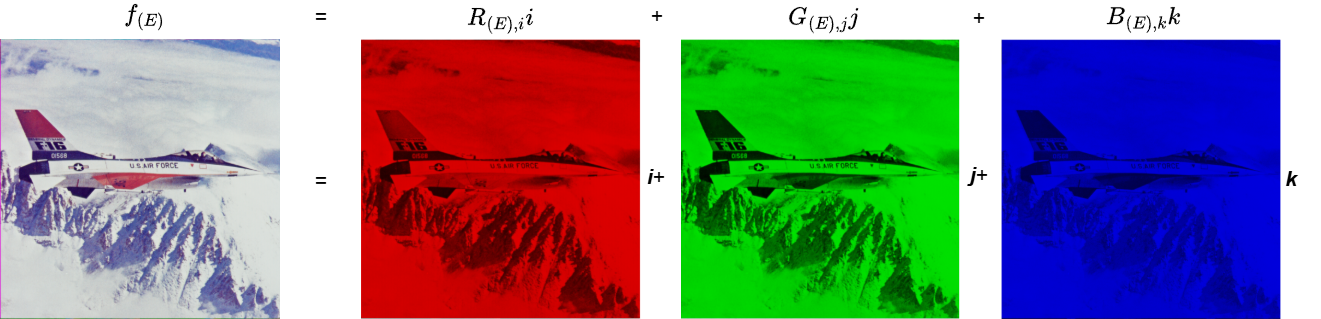
\includegraphics[scale=0.18]{images/airplane_el_rep.png}
\end{figure}
\end{frame}

\begin{frame}{$p$ Hiperparametresi}
\bglogo
\begin{block}{$p$ Parametresinin Önemi}
2023 yılında tamamlanan 121F289 numaralı ``Eliptik Kuaterniyon Matris Teorisinin Geliştirilmesi ve Uygulamaları'' projesinde elde edilen ${{A}_{\left( E \right)}}{{X}_{\left( E \right)}}={{B}_{\left( E \right)}}$ matris denkleminin en küçük normlu en küçük kareler çözümünün $p$ ve $m$ değerlerine göre hata yüzeyi şekildeki gibidir. Yüzey üstündeki kırmızı noktalar problemin çözümünü optimal yapan $p$ değerlerini göstermektedir. $p$ değeri, geliştirilecek algoritmanın \textbf{tüm birimlerini aynı anda etkileyen hem performans hem de güvenlik parametresi} olarak karşımıza çıkmaktadır.
\end{block}

\begin{figure}[h]
    \centering
    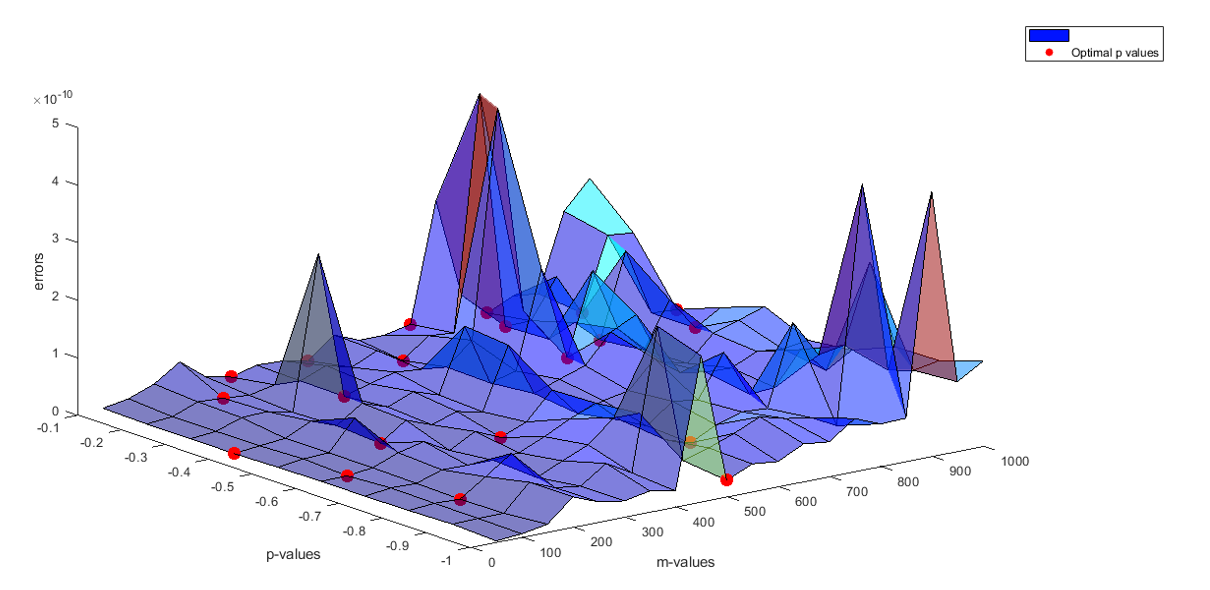
\includegraphics[scale=0.18]{images/hata_yuzeyi.png}
\end{figure}
\end{frame}

\begin{frame}{Çok Katmanlı Güvenlik Mimarisi}
\bglogo
\textbf{QuatMark-EQCore'un Dört Katmanlı Güvenlik Yapısı:}

\begin{enumerate}
\item \textbf{$p$ Anahtarı:} İşlemin gerçekleşeceği eliptik uzay (gizli hiperparametre)
\item \textbf{Arnold Karıştırma:} Damga verisinin uzamsal permütasyonu
\item \textbf{Kaotik Şifreleme:} Karıştırılmış damganın kaotik haritalarla şifrelenmesi (Logistic, Tent, PWLCM)
\item \textbf{SHA-2 Tabanlı Konumlandırma:} Gizli anahtara bağlı pseudo-rastgele blok seçimi
\end{enumerate}

\vspace{0.3cm}

\begin{block}{Avantajlar}
\begin{itemize}
\item Yetkisiz erişime karşı çok katmanlı savunma -- her katman ayrı anahtar gerektirir.
\item Saldırgan, hangi cebirsel uzayda ($p$) işlem yapıldığını bilemez.
\item Damga deseninin tahmin edilebilirliği minimize edilir.
\item Derin öğrenme tabanlı saldırılara karşı yapısal direnç sağlar.
\end{itemize}
\end{block}
\end{frame}

\begin{frame}
\frametitle{Arnold Karıştırma Algoritması}
\bglogo
\begin{block}{Tanım}
Arnold'un Dönüşümü, birim kare (genellikle bir görüntü) üzerinde uygulanan \textbf{kaotik} bir dönüşümdür. Görüntüdeki piksellerin yerini belirli bir kurala göre defalarca değiştirerek karıştırmak için kullanılır.
\end{block}

\begin{block}{Matematiksel Formül ($M \times N$ Görüntü için)}
$M \times N$ boyutlarındaki bir görüntüde yer alan $(x, y)$ koordinatındaki bir pikselin, bir sonraki iterasyondaki yeni $(x', y')$ konumu:
$$
\begin{pmatrix} x' \\ y' \end{pmatrix} =
\begin{pmatrix} 1 & 1 \\ 1 & 2 \end{pmatrix}
\begin{pmatrix} x \\ y \end{pmatrix} \;\; (\bmod\, M, \bmod\, N)
$$
\end{block}
\end{frame}

\begin{frame}
\frametitle{Kaotik Sistemler}
\bglogo
Kaotik sistemler aşağıdaki özelliklere sahip olmaktadır:
\begin{itemize}
\item Sözde rasgelelik
\item Başlangıç değerlerine karşı yüksek hassasiyet
\item Doğrusal olmama
\end{itemize}

\vfill

\begin{block}{Lojistik Haritası}
$$ X_{k} = \mu X_{k-1}(1 - X_{k-1}) $$
\begin{itemize}
\item $X_k \in (0,1)$
\item $\mu$ (kontrol parametresi) için kaosa geçiş değeri:
\item $\mu \approx 3.5699456...$
\end{itemize}
\end{block}
\end{frame}

\begin{frame}
\frametitle{Kaotik Şifreleme ile Görüntü İşleme}
\bglogo
\begin{block}{Amaç}
Kaotik şifreleme ile görüntünün istatistiksel saldırılara karşı daha etkili biçimde direnmesi sağlanır. Proje kapsamında \textbf{Logistic Map, Tent Map ve PWLCM} tabanlı kaotik şifreleme katmanları değerlendirilecektir.
\end{block}

\begin{block}{Adımlar}
\begin{enumerate}
\item Damga görüntüsü ($M \times N$ boyutlarında) alınır.
\item $M$ ve $N$ değerleri girdi olarak kullanılır.
\item Kaotik harita ile $R$ matrisi oluşturulur.
\item Bozucu matris ($R_1$) hesaplanır:
$$ R_1(i,j) = \text{round}(1000 \cdot R(i,j)) \pmod{255} $$
\item Damga verisi ile $R_1$, XOR işlemine tabi tutulur.
\end{enumerate}
\end{block}
\end{frame}

\begin{frame}
\frametitle{Hash Fonksiyonları}
\bglogo
\begin{block}{Tanım}
Bir hash fonksiyonu, herhangi bir veriyi alıp onu sabit boyutlu, benzersiz bir özet dizisine dönüştüren matematiksel bir işlemdir.
\end{block}

\begin{block}{Yaygın Algoritmalar ve Güvenlik Durumları}
\begin{itemize}
\item MD5 (128-bit) -- \textit{Güvensiz (çakışmalara çok açık)}
\item SHA-1 (160-bit) -- \textit{Güvensiz (çakışma saldırılarına açık)}
\item \textbf{SHA-2 (256/512-bit)} -- \textit{Güvenli, günümüzde endüstri standardı (proje seçimi)}
\item SHA-3 (256/512-bit) -- \textit{Güvenli, SHA-2'ye modern alternatif}
\end{itemize}
\end{block}
\end{frame}

\begin{frame}
\frametitle{Metodoloji: SHA-2 Tabanlı PRNG Tohumlama}
\bglogo
\begin{block}{Yaklaşım}
QuatMark-EQCore çekirdeği, host görüntüden hangi blokların seçileceğini belirlemek için bir Sözde Rastgele Sayı Üreteci (PRNG) kullanır.
\vfill
PRNG'nin "tohum" (seed) değeri, kullanıcı anahtarına (key) uygulanan \textbf{SHA-2 (SHA-256)} hash fonksiyonunun çıktısından elde edilir.
\end{block}

\begin{alertblock}{Neden SHA-2?}
\begin{itemize}
%\item Eski projedeki MD5 yaklaşımının çakışma (collision) zafiyeti tamamen elimine edildi.
\item SHA-2'nin kriptografik sağlamlığı ve çarpışma direnci, gömme konumlarının tahmin edilemezliğini güvence altına alır.
\item Karşılaştırmalı analizler için gerektiğinde MD5/SHA-1/SHA-3 çıktılarıyla algoritmanın sağlamlığı ölçülecektir.
\end{itemize}
\end{alertblock}
\end{frame}

\begin{frame}
\frametitle{İndeks Seçme Aşamaları (1/2)}
\bglogo
\begin{block}{Adım 1: Hash Çıktısı}
Anahtar, SHA-2 (SHA-256) fonksiyonuna verilir; 64 karakter uzunluğunda 16'lık (hexadecimal) tabanda hash çıktısı alınır.
\end{block}

\begin{block}{Adım 2: Tabana Dönüştürme}
Üretilen hex tabanlı sayı, 10'luk (decimal) tabana çevrilir.
\end{block}

\begin{block}{Adım 3: Tohum (Seed) Oluşturma}
Bu 10'luk tabandaki sayı, sözde-rastgele sayı üretecinin tohumu (seed) olarak kullanılır.
\end{block}
\end{frame}

\begin{frame}
\frametitle{İndeks Seçme Aşamaları (2/2)}
\bglogo
\begin{block}{Adım 4: Rastgele Blok Seçimi Algoritması}
N adet rasgele blok seçilir.

\textbf{Sözde-Kod (Pseudo-code):}

\texttt{current\_val = hash\_val (tohum)} \\
\texttt{selected\_blocks = set()} \\
\texttt{while (döngü devam ettikçe)} \\
\hspace{1cm} \texttt{idx = current\_val \% N} \\
\hspace{1cm} \texttt{selected\_blocks.append(block[idx])} \\
\hspace{1cm} \texttt{current\_val = next(CSPRNG\_state)}
\vfill
(Üretici olarak ChaCha20 / HMAC-DRBG / AES-CTR DRBG değerlendirilecektir.)
\end{block}
\end{frame}

\begin{frame}
\frametitle{PRNG Alternatifleri ile İndeks Üretimi}
\bglogo
\begin{block}{Neden Klasik LCG Değil?}
LCG hızlıdır; ancak \textbf{tahmin edilebilirlik} ve \textbf{örüntü/korelasyon} nedeniyle saldırı altında zayıftır.
\end{block}

\begin{block}{Kullanılabilecek Modern Alternatifler}
\begin{itemize}
\item \textbf{CSPRNG/DRBG:} ChaCha20, AES-CTR, HMAC/Hash-DRBG (öncelikli adaylar)
\item \textbf{Modern PRNG:} PCG, xoshiro/xoroshiro, SplitMix64
\item \textbf{Baz çizgi:} Mersenne Twister (MT19937)
\end{itemize}
\end{block}
\end{frame}

\begin{frame}{Damgalama Süreci}
\bglogo
\begin{enumerate}
\item \textbf{Ön İşleme:}
\begin{itemize}
\item Damga verisi Arnold dönüşümü ile karıştırılır.
\item Kaotik şifreleme uygulanır.
\item 8 bitlik ikili dizilere dönüştürülür.
\end{itemize}

\item \textbf{Gömme:}
\begin{itemize}
\item Ana görüntü $4 \times 4$ eliptik kuaterniyon bloklarına ayrılır.
\item \textbf{SHA-2} tabanlı pseudo-rastgele algoritma ile bloklar seçilir.
\item Her bloğa eliptik kuaterniyon QR ayrışımı uygulanır.
\item Damga bitleri $R(1,4)$ elemanına kuantizasyon ile gömülür.
\end{itemize}

\item \textbf{Çıkarma (Kör):}
\begin{itemize}
\item Damgalı görüntüden aynı anahtarla bloklar tespit edilir.
\item QR ayrışımı ve ters kuantizasyon uygulanır.
\item Ters Arnold ve kaotik deşifreleme ile orijinal damga elde edilir.
\end{itemize}
\end{enumerate}
\end{frame}

\begin{frame}{Damga Gömme Prosedürü}
\processvisualwithfallback{images/damga_gomme_proseduru.png}{Damga Gömme Prosedürü}
{Damga ön işleme, host görüntü işleme, QR ayrışımı, $R_{1,4}$ elemanına gömme ve ters QR inşa adımları tek akışta gösterilir.}{images/GORSEL1.png}
\end{frame}

\begin{frame}{Damga Çıkarma Prosedürü}
\processvisualwithfallback{images/damga_cikarma_proseduru.png}{Damga Çıkarma Prosedürü}
{Kör çıkarma yaklaşımıyla damgalı görüntü ve gizli anahtarlar üzerinden QR ayrışımı, bit çıkarma, ters şifreleme ve orijinal host geri kazanımı gösterilir.}{images/GORSEL2.png}
\end{frame}

\begin{frame}{Performans Kriterleri}
\bglogo
\textbf{Algılanamazlık (Imperceptibility):}
\begin{itemize}
\item PSNR (Peak Signal-to-Noise Ratio) $>$ 40 dB
\item SSIM (Structural Similarity Index) $>$ 0,98
\item Damgalı görüntü orijinalden ayırt edilemez.
\end{itemize}

\vspace{0.3cm}

\textbf{Sağlamlık (Robustness):}
\begin{itemize}
\item Geleneksel saldırılara karşı $NC \geq 0,98$
\begin{itemize}
\item JPEG sıkıştırma (kalite faktörü $\geq 70$)
\item Geometrik dönüşümler ($\pm 10$\textdegree~döndürme, $\pm 10\%$ ölçeklendirme)
\item Kırpma (\%80'e kadar), gürültü (SNR $\geq 30$ dB)
\item Parlaklık ayarı ($\pm 20\%$), filtreleme/histogram eşitleme
\end{itemize}
\item Derin öğrenme saldırılarına karşı $NC \geq 0,95$ (PSNR $> 35$ dB, SSIM $> 0,95$ saldırı görüntüleri için bile)
\end{itemize}
\end{frame}

% =====================================================================
% Bölüm 4: Rekabet Analizi
% =====================================================================
% \section{Rekabet Analizi}

% \begin{frame}{Rakip Karşılaştırması -- 6 Rakip}
% \bglogo
% \scriptsize
% \begin{table}
% \centering
% \begin{tabular}{p{2.4cm}p{2.0cm}p{1.6cm}p{1.6cm}p{1.5cm}p{1.5cm}p{1.5cm}}
% \toprule
% \textbf{Kriter} & \textbf{QuatMark-EQCore} & \textbf{Digimarc} & \textbf{IMATAG} & \textbf{Verimatrix/Irdeto} & \textbf{MarkAny} & \textbf{Google SynthID} \\
% \midrule
% Gömme Dön. & EQ QR Ayrışımı & DCT/DWT & SVD & Spread-Spectrum & DCT/DWT & NN Enjeksiyon \\
% Temsil Uzayı & 4-D EQ Matris & Reel (frekans) & Reel (sing.) & Reel & Reel/karm. & NN gizli uzay \\
% Renk Kanalı & \textbf{Bütünleşik} & Ayrıştırmalı & Ayrıştırmalı & Ayrıştırmalı & Ayrıştırmalı & Sınırlı \\
% Blok Seçimi & SHA-2 + kaotik & Statik & Kısmen adp. & Oturum anh. & Statik & Öğrenilmiş \\
% Şifreleme & Kaotik+SHA-2+Arnold & AES & AES & Oturum krip. & DRM anh. & Kapalı \\
% Kör Damgalama & \textbf{Evet} & Evet & Evet & Evet & Kısmi & Hayır \\
% DL Saldırı Sav. & \textbf{Var} & Yok & Yok & Yok & Yok & Kapalı \\
% Yerli/Milli & \textbf{Evet} & Hayır & Hayır & Hayır & Hayır & Hayır \\
% \bottomrule
% \end{tabular}
% \end{table}

% \textbf{Belirgin farklılaşma:} Kanal-bütünleşik işleme + kamuya açık DL savunması + yerli teknoloji.
% \end{frame}

% \begin{frame}{QuatMark-Standart Çekirdek vs. EQCore}
% \bglogo
% \scriptsize
% \begin{table}
% \centering
% \begin{tabular}{p{4.5cm}p{4.5cm}p{4.5cm}}
% \toprule
% \textbf{Teknik Özellik} & \textbf{Yeni: QuatMark-EQCore} & \textbf{Mevcut: Standart Çekirdek} \\
% \midrule
% İşlem Alanı & EQ QR ayrışımı (dönüşüm uzayı) & Reel matris QR ayrışımı \\
% Renk Kanalı İşleme & Bütünleşik, senkronize & Bağımsız (kanal başına) \\
% Çalışma Uzayı & 4-boyutlu EQ cebiri & Reel sayı uzayı \\
% Damga Ön-İşleme: Kaotik Şifreleme & Var & Yok \\
% Damga Ön-İşleme: Arnold Karıştırma & Var & Yok \\
% Renk Korelasyonu Kaybı & Ortadan kaldırılmış & Mevcut \\
% Damga Asenkronizasyonu & Ortadan kaldırılmış & Mevcut \\
% Blok Seçimi & SHA-2 tabanlı (anahtar bağımlı) & numpy.random \\
% Güvenlik Katmanı Sayısı & \textbf{4 katman} ($p$+SHA-2+Arnold+kaotik) & Tek katman \\
% \bottomrule
% \end{tabular}
% \end{table}
% \end{frame}

% =====================================================================
% Bölüm 5: Uygulama Alanları
% =====================================================================
\section{Uygulama Alanları ve Hedef Kitle}

\begin{frame}{Hedef Sektörler}
\bglogo
\begin{enumerate}
\item \textbf{Medya ve Yayıncılık:}
\begin{itemize}
\item Haber ajansları, fotoğrafçılar, prodüksiyon şirketleri
\item Telif hakkı koruması ve dijital korsanlığın önlenmesi
\end{itemize}

\item \textbf{Savunma Sanayii:}
\begin{itemize}
\item Askeri teknoloji kuruluşları, istihbarat birimleri
\item İHA/uydu görüntülerinin bütünlük kontrolü
\item Sızıntı tespiti ve kaynak belirleme
\end{itemize}

\item \textbf{Sağlık Bilişimi:}
\begin{itemize}
\item Hastaneler, tıbbi görüntüleme merkezleri
\item Tıbbi görüntülerin (MR/CT/röntgen) orijinallik doğrulaması -- KVKK/HIPAA uyumu
\end{itemize}

\item \textbf{Adli Bilişim ve Hukuk:}
\begin{itemize}
\item Emniyet, adli tıp, mahkeme/hukuk büroları
\item Dijital delillerin kriptografik bütünlük doğrulaması
\end{itemize}
\end{enumerate}
\end{frame}

\begin{frame}{Uygulama Senaryoları (Özet)}
\bglogo
\begin{enumerate}
\item \textbf{Telif Hakkı Koruması:}
\begin{itemize}
\item Dijital içeriğe telif bilgisi gömülür.
\item İzinsiz kullanım tespit edilir; yasal delil niteliği taşır.
\end{itemize}

\item \textbf{Kimlik Doğrulama:}
\begin{itemize}
\item İçeriğin orijinalliği teyit edilir.
\item Manipülasyon tespit edilir; güvenilirlik sağlanır.
\end{itemize}

\item \textbf{Sızıntı Tespiti:}
\begin{itemize}
\item Her kopyaya benzersiz damga eklenir.
\item Sızıntı kaynağı kesin olarak belirlenir.
\item İçeriden tehditler önlenir.
\end{itemize}
\end{enumerate}
\end{frame}

% =====================================================================
% Bölüm 6: Ürün Yapısı ve Ticarileşme
% =====================================================================
\section{Ürün Yapısı ve Ticarileşme}

\begin{frame}{QuatMark Ürün Yapısı (Mevcut)}
\begin{alertblock}{Önemli Not}
SaaS platformu, RESTful API ve ödeme altyapısı, şirketimizin \textbf{öz kaynaklarıyla halihazırda geliştirilmiş} ve aktif olarak hizmet vermektedir. Yeni proje (190871) yalnızca bu ürünün \textbf{çekirdeğini yenilemeyi} hedefler.
\end{alertblock}

\begin{columns}
\column{0.5\textwidth}
\begin{block}{SaaS Platform (mevcut)}
\textbf{Web Tabanlı Hizmet}
\begin{itemize}
\item Kullanıcı dostu arayüz
\item Manuel damgalama
\item Abonelik modeli
\item İstatistik ve raporlama
\end{itemize}
\end{block}

\column{0.5\textwidth}
\begin{block}{API Entegrasyonu (mevcut)}
\textbf{Geliştirici Araçları}
\begin{itemize}
\item RESTful API
\item Otomatik damgalama
\item Sistem entegrasyonu
\item Ölçeklenebilir altyapı
\end{itemize}
\end{block}
\end{columns}

\textbf{Proje Çıktısı:} Yeni EQCore çekirdeğinin bu mevcut ürüne sürümleme ve pilot doğrulama ile entegrasyonu (İP3).
\end{frame}

\begin{frame}{İş Modeli ve Gelir Kaynakları}
\bglogo
\textbf{1. SaaS Abonelik (B2B + B2C):}
\begin{itemize}
\item Yıllık $\sim$2.400 TL + KDV (aylık 200 TL)
\item Hedef: 1. yıl 80, 3. yıl 600, 5. yıl 1.800 abone
\item Brüt kâr marjı $\sim\%87,5$ (birim maliyet 300 TL/yıl)
\end{itemize}

\textbf{2. Kurumsal API Lisanslama (B2B):}
\begin{itemize}
\item Yıllık $\sim$180.000 TL + KDV
\item Hedef: 1. yıl 2, 3. yıl 8, 5. yıl 18 lisans
\item Brüt kâr marjı $\sim\%83,3$ (birim maliyet 30.000 TL)
\end{itemize}

\textbf{3. Fikri Mülkiyet Lisanslama:} Patent tabanlı pasif gelir.

\textbf{4. Türev Ar-Ge ve Danışmanlık:} Kriptografi/veri gizleme uzmanlığının ticarileşmesi.
\end{frame}

\begin{frame}{Pazar Analizi ve Pazar Payı Hedefleri}
\bglogo
\small
\begin{block}{Küresel Pazar (Grand View Research)}
\begin{itemize}
\item \textbf{Genel dijital damgalama pazarı:} 2024'te 1,45 milyar USD; 2033'te 3,80 milyar USD; CAGR \%11,4.
\item \textbf{AI watermarking pazarı:} 2024'te 427,2 milyon USD; 2033'te \textbf{3,07 milyar USD}; CAGR \textbf{\%25,3}.
\item YZ Yasası Madde 50 ve C2PA uyumu, hızlı büyüyen AI watermarking segmentini stratejik hedef pazar hâline getirmektedir.
\end{itemize}
\end{block}

\textbf{Pazar Payı Hedefleri (Türkiye):}
\begin{table}
\centering
\begin{tabular}{lcc}
\toprule
\textbf{Yıl} & \textbf{Hedef Pay} & \textbf{Strateji} \\
\midrule
1. Yıl & \%2-3 & Pilot referans müşteriler \\
3. Yıl & \%8-10 & Pazar penetrasyonu \\
5. Yıl & \%15-20 & Pazar liderliği + uluslararası açılım \\
\bottomrule
\end{tabular}
\end{table}

\textbf{Kâra Geçiş:} Proje başlangıcından itibaren \textbf{40. ay} (Ekim 2029).
\end{frame}

% =====================================================================
% Bölüm 7: İş Planı
% =====================================================================
\section{Proje İş Planı}

\begin{frame}{İş Paketleri -- Genel Bakış (3 İP)}
\bglogo
\begin{block}{İP1: Teorik Altyapı (01.06.2026 -- 30.11.2026, 6 ay)}
Eliptik kuaterniyon uzayı için Householder dönüşümü ve QR ayrışımı teorilerinin elde edilmesi; \texttt{EQquaternion.py} Python modülü.
\end{block}

\begin{block}{İP2: Damgalama Modeli (01.12.2026 -- 30.04.2027, 5 ay)}
Tüm renk bileşenlerini bütünleşik ve senkronize işleyen, çok katmanlı güvenlik mimarisine sahip damgalama modelinin ortaya konması; performans ve saldırı dayanıklılığı testleri.
\end{block}

\begin{block}{İP3: Entegrasyon ve Pilot (01.05.2027 -- 30.09.2027, 5 ay)}
QuatMark-EQCore çekirdeğinin mevcut QuatMark ürününe entegrasyonu, sürümleme, dokümantasyon ve pilot kullanıcı doğrulaması.
\end{block}

\textbf{Toplam:} 13 somut ve ölçülebilir ara çıktı, tüm faaliyetler kuruluş bünyesinde yürütülür.
\end{frame}

\begin{frame}{İş Paketi 1: Teorik Altyapı}
\bglogo
\textbf{Faaliyetler:}
\begin{itemize}
\item Eliptik kuaterniyon cebiri ve izomorfizm yapısının incelenmesi
\item Eliptik kuaterniyon vektör uzayında \textbf{Householder dönüşümünün} özgün formülasyonu
\item $m \times n$ boyutlu eliptik kuaterniyon matrisleri için \textbf{QR ayrışımı teorisi}
\item Algoritma tasarımı ve pseudo kod yazımı (4$\times$4 matris için $<$ 0,184 ms)
\item \texttt{EQquaternion.py} Python modülünün geliştirilmesi
\item Akademik dokümantasyon ve teorik doğrulama
\end{itemize}

\textbf{Ara Çıktılar (4):}
\begin{enumerate}
\item Householder formülasyon raporu (31.08.2026)
\item QR ayrışımı teorisi ve algoritma dokümanı (31.10.2026)
\item Optimal $p$ aralığı analiz raporu (30.11.2026)
\item \texttt{EQquaternion.py} modülü (30.11.2026)
\end{enumerate}
\end{frame}

\begin{frame}{İş Paketi 2: Damgalama Modeli}
\bglogo
\textbf{Faaliyetler:}
\begin{itemize}
\item Arnold + kaotik şifreleme + SHA-2 katmanlarının \texttt{EQquaternion.py}'a entegrasyonu
\item Damga gömme/çıkarma prosedürlerinin elde edilmesi (R(1,4) kuantizasyonu)
\item Algılanamazlık testleri: PSNR $>$ 40 dB, SSIM $>$ 0,98
\item Geleneksel saldırı dayanıklılığı testleri: NC $\geq$ 0,98
\item Derin öğrenme tabanlı saldırı testleri: NC $\geq$ 0,95
\item Kör/sağlam damgalama yöntemleriyle karşılaştırma
\end{itemize}

\textbf{Ara Çıktılar (5):}
\begin{enumerate}
\item Çok katmanlı güvenlik mimarisi raporu (31.01.2027)
\item Damga gömme/çıkarma uygulama raporu (28.02.2027)
\item Algılanamazlık (PSNR/SSIM) raporu (31.03.2027)
\item Saldırı dayanıklılığı (NC) raporu (30.04.2027)
\item Bütünleşik damgalama modeli (30.04.2027)
\end{enumerate}
\end{frame}

\begin{frame}{İş Paketi 3: Entegrasyon ve Pilot Doğrulama}
\bglogo
\textbf{Faaliyetler:}
\begin{itemize}
\item Modüler entegrasyon arayüzü tasarımı ve API sarmalayıcı geliştirimi
\item Birim testleri ve entegrasyon testleri (\textbf{IEEE 829} standardı)
\item Saldırı dayanıklılığı + performans doğrulama testleri
\item Sürüm yönetimi (Git/GitHub) ve teknik dokümantasyon
\item Medya, savunma, sağlık bilişimi sektörlerinden \textbf{pilot kullanıcılarla} doğrulama
\item Akademik yayın ve patent başvuruları için temel referans hazırlığı
\end{itemize}

\textbf{Ara Çıktılar (4):}
\begin{enumerate}
\item Entegrasyon arayüzü tasarım dokümanı (01.06.2027)
\item Birim ve entegrasyon test raporu (01.07.2027)
\item Saldırı/kalite test raporu (01.08.2027)
\item Pilot doğrulama raporu ve nihai dokümantasyon (01.09.2027)
\end{enumerate}
\end{frame}

\begin{frame}{Proje Ekibi (3 Kişi)}
\bglogo
\begin{columns}[t]
\column{0.5\textwidth}
\textbf{Ana Personel:}
\begin{itemize}
\item \textbf{Doç. Dr. Hidayet Hüda Kösal}
\begin{itemize}
\item Teknoloji Direktörü, Ar-Ge Sorumlusu
\item Proje yürütücüsü, teorik altyapı ve bilimsel koordinasyon
\item Adam-Ay Oranı: 0,6
\end{itemize}

\vspace{0.3cm}

\item \textbf{Yazılım Geliştirme Uzmanı (Mühendis)}
\begin{itemize}
\item Algoritma kodlama, \texttt{EQquaternion.py} geliştirme
\item Sistem entegrasyonu ve test
\item Adam-Ay Oranı: 0,7
\end{itemize}
\end{itemize}

\column{0.5\textwidth}
\begin{itemize}
\item \textbf{Araştırmacı (Temel Bilimci)}
\begin{itemize}
\item Matematiksel formülasyon, teorik destek ve analiz
\item Adam-Ay Oranı: 0,7
\end{itemize}
\end{itemize}

\vfill

\begin{block}{Toplam Adam-Ay}
\textbf{30,72 adam-ay} (eski projeye göre \%43 azalma)
\end{block}

\begin{block}{Dış Hizmet}
Yalnızca \textbf{Akademik Danışmanlık} (Sakarya Uygulamalı Bilimler Üniversitesi)
\end{block}
\end{columns}
\end{frame}

% =====================================================================
% Bölüm 8: Bütçe
% =====================================================================
\section{Proje Bütçesi}

\begin{frame}{Bütçe Dağılımı}
\bglogo
\begin{table}
\centering
\small
\begin{tabular}{lrrr}
\toprule
\textbf{Maliyet Kalemi} & \textbf{Tutar (TL)} & \textbf{Oran} & \textbf{Eski Proje (TL)} \\
\midrule
Personel Giderleri & $\sim$1.631.000 & $\sim$\%88,6 & $\sim$4.847.000 \\
Hizmet Alımları (Akademik Danışmanlık) & 160.000 & $\sim$\%8,7 & 2.790.000 \\
Seyahat Giderleri & 50.000 & $\sim$\%2,7 & 100.000 \\
Alet/Teçhizat/Yazılım & 0 & \%0,0 & 250.000 \\
Yurtiçi Ar-Ge ve Test & 0 & \%0,0 & 150.000 \\
\midrule
\textbf{TOPLAM} & \textbf{$\sim$1.841.233} & \textbf{\%100} & \textbf{$\sim$8.137.000} \\
\bottomrule
\end{tabular}
\end{table}

\vspace{0.3cm}

%\textbf{Eski projeye göre \%77 azalma.} Bütçe doğrudan Ar-Ge değer zincirine yoğunlaştırılmıştır; G-THOHT yazılım hizmeti ve ASC hukuk danışmanlığı tamamen çıkarılmıştır.
\end{frame}

\begin{frame}{Eski Projeyle Karşılaştırma -- Genel}
\bglogo
\scriptsize
\begin{table}
\centering
\begin{tabular}{p{4cm}p{4cm}p{4cm}}
\toprule
\textbf{Kriter} & \textbf{Eski Proje (3251897)} & \textbf{Yeni Proje (190871)} \\
\midrule
Program & TÜBİTAK 1501 & \textbf{TÜBİTAK 1507 KOBİ Ar-Ge} \\
Odak & Çekirdek + SaaS + API + Pazarlama & \textbf{Yalnızca yeni nesil çekirdek} \\
SaaS/API Altyapısı & Geliştirilecekti & Öz kaynakla halihazırda mevcut \\
Süre & 18 ay & \textbf{16 ay} \\
Adam-Ay & 53,58 & \textbf{30,72} (\%43 azalma) \\
Bütçe & $\sim$8.137.000 TL & \textbf{$\sim$1.841.000 TL} (\%77 azalma) \\
Personel Sayısı & 5 kişi & \textbf{3 kişi} \\
İş Paketi & 4 İP & \textbf{3 İP} \\
Ara Çıktı & 4 adet & \textbf{13 adet} \\
THS Hedef & THS3 $\rightarrow$ THS7 & THS3 $\rightarrow$ \textbf{THS8} \\
Hash Algoritması & MD5 & \textbf{SHA-2 (SHA-256)} \\
Rakip Kıyaslama & 3 rakip & \textbf{6 rakip + 12 kriter} \\
Dış Hizmet & G-THOHT, ASC Hukuk & Sadece akademik danışmanlık \\
Ticarileşme & 1-3 yıl & \textbf{0-1 yıl} (mevcut ürün) \\
\bottomrule
\end{tabular}
\end{table}
\end{frame}

% =====================================================================
% Bölüm 9: Riskler
% =====================================================================
\section{Risk Yönetimi}

\begin{frame}{Potansiyel Riskler ve Önlemler}
\bglogo
\scriptsize
\begin{table}
\centering
\begin{tabular}{p{3.8cm}p{4.2cm}p{4.2cm}}
\toprule
\textbf{Risk} & \textbf{Önlem} & \textbf{B Planı} \\
\midrule
Teorinin performans hedeflerine ulaşamaması & $\{e_1,e_2\}$ idempotent bazı kullanımı & $\{1,i,j,k\}$, $\{1,j\}$ bazlarıyla karşılaştırma \\
Arnold anahtar zafiyeti & 4 katmanlı güvenlik mimarisi & Genelleştirilmiş Arnold dönüşümü \\
Derin öğrenme saldırılarına direnç & Kanal-bütünleşik EQ + kaotik şifreleme & Çifte Arnold karıştırma ($K_i, K_j$) \\
Saldırılar sonrası NC hedefinin altında kalma & EQ tabanlı yeni kuantizasyon & Reed-Solomon hata düzeltme kodları \\
Patent süreci uzaması veya çakışma & Patent vekili + hukuk danışmanlığı & Ticari sır olarak koruma \\
Bütçe yetersizliği & Aylık bütçe-harcama takibi & Şirket öz kaynakları ile karşılama \\
Pazar kabulü & Pilot referans müşteriler, akademik yayın & Stratejik ortaklıklar, kamu ihaleleri \\
\bottomrule
\end{tabular}
\end{table}
\end{frame}

% =====================================================================
% Bölüm 10: Beklenen Çıktılar
% =====================================================================
\section{Beklenen Çıktılar ve Etkiler}

\begin{frame}{Proje Çıktıları}
\bglogo
\textbf{Teknolojik Çıktılar:}
\begin{itemize}
\item Eliptik kuaterniyon Householder dönüşümü ve QR ayrışımı teorisi
\item \texttt{EQquaternion.py} Python modülü
\item QuatMark-EQCore damgalama çekirdeği
\item Mevcut QuatMark ürününe entegre edilmiş, pilot doğrulanmış sürüm
\end{itemize}

\textbf{Bilimsel Çıktılar:}
\begin{itemize}
\item Etki faktörü yüksek uluslararası dergi/konferans yayınları
\item Ulusal ve uluslararası patent başvuruları
\item Matematik ve kriptografi literatürüne özgün katkı
\end{itemize}

\textbf{Ticari Çıktılar:}
\begin{itemize}
\item Yenilenmiş çekirdek üzerinden artırılmış SaaS/API gelirleri
\item Yerli ve milli teknoloji, ihracat potansiyeli (USD bazında)
\end{itemize}
\end{frame}

\begin{frame}{Ekonomik ve Ulusal Kazanımlar}
\bglogo
\textbf{Ekonomik Katkılar:}
\begin{itemize}
\item Yerli ve milli dijital damgalama teknolojisi
\item İthal ikamesi (Digimarc/IMATAG/MarkAny vb. yerine yerli alternatif)
\item Yüksek katma değerli ürün, ihracat potansiyeli
\end{itemize}

\textbf{Bilimsel ve Teknolojik İlerleme:}
\begin{itemize}
\item Yeni matematiksel teorilerin geliştirilmesi
\item Veri güvenliği alanında yeni uygulamalar
\item Literatüre özgün katkı (akademik boşluğun doldurulması)
\end{itemize}

\textbf{İnsan Kaynağı Gelişimi:}
\begin{itemize}
\item Nitelikli araştırmacı ve mühendis yetiştirilmesi
\item Disiplinler arası bilgi birikimi (matematik + kriptografi + yazılım)
\item Ulusal rekabet gücünün artırılması
\end{itemize}
\end{frame}

\begin{frame}{Öncelikli Alan Uyumu}
\bglogo
\begin{block}{Çağrı Metni Öncelikli Alanı}
\textbf{Gerçek dışı çoklu ortam içeriklerin (görüntü, video ve ses) son kullanıcı cihazlarında tespit edilebilmesine ve önlenebilmesine yönelik teknolojiler.}
\end{block}

\textbf{Doğrudan Uyum:}
\begin{itemize}
\item Deepfake/generative AI içeriklerine karşı kriptografik kimlik doğrulama
\item Tespit (damga doğrulama) ve önleme (alıcıya özel sızıntı izleme) işlevleri
\item Eliptik kuaterniyon temelli özgün matematiksel altyapı
\item Yerli ve milli teknoloji ile dışa bağımlılığın azaltılması
\end{itemize}

\textbf{12. Kalkınma Planı Uyumu:} Bilişim ve İletişim Teknolojileri öncelikli alanı; savunma için siber güvenlik, veri kaçağı önleme ve içerik bütünlüğü altyapısı.
\end{frame}

\begin{frame}{Sosyal Fayda}
\bglogo
\textbf{Dezenformasyonla Mücadele:}
\begin{itemize}
\item Deepfake ve sahte haberlere karşı kriptografik içerik doğrulama
\item Toplumsal güvenin ve bilgi güvenilirliğinin korunması
\end{itemize}

\textbf{Sağlık ve Adalet Sistemine Güven:}
\begin{itemize}
\item Tıbbi görüntülerin bütünlüğüyle hatalı teşhislerin önlenmesi
\item Hukuki süreçlerde dijital delillerin orijinalliğinin doğrulanması
\end{itemize}

\textbf{Ulusal Güvenlik ve Teknolojik Egemenlik:}
\begin{itemize}
\item Savunma sanayiinde hassas görsel verilerin bütünlüğü
\item Kritik altyapılarda yabancı çözüme bağımlılığın azaltılması
\end{itemize}
\end{frame}

% =====================================================================
% Bölüm 11: Sonuç
% =====================================================================
\section{Sonuç ve Vizyon}

\begin{frame}{Proje Sonuçları -- Özet}
\bglogo
\begin{block}{Teknolojik İnovasyon}
Eliptik kuaterniyon tabanlı, çok katmanlı güvenlik mimarisine sahip, derin öğrenme saldırılarına karşı dayanıklı, yüksek performanslı yeni nesil dijital damgalama çekirdeği.
\end{block}

\textbf{Ana Başarı Kriterleri:}
\begin{itemize}
\item Teorik altyapının literatüre özgün biçimde kazandırılması
\item EQCore çekirdeğinin geliştirilip mevcut ürüne entegre edilmesi
\item PSNR $>$ 40 dB, SSIM $>$ 0,98, NC $\geq$ 0,98 (geleneksel), NC $\geq$ 0,95 (DL)
\item Yerli ve milli teknoloji üretimi, patent koruması
\end{itemize}

\textbf{Beklenen Etkiler:}
\begin{itemize}
\item Dijital güvenlik alanında teknolojik ilerleme
\item Stratejik sektörlerde dışa bağımlılığın azalması
\item Bilimsel literatüre özgün katkı, yüksek katma değer
\end{itemize}
\end{frame}

\begin{frame}{Gelecek Vizyonu}
\bglogo
\textbf{Kısa Vadeli Hedefler (1-2 Yıl):}
\begin{itemize}
\item Projenin başarıyla tamamlanması (Eylül 2027)
\item EQCore çekirdeğinin mevcut QuatMark ürününe lansmanı
\item Pilot referans müşterilerin kazanılması
\item Patent başvurularının tamamlanması
\end{itemize}

\textbf{Orta Vadeli Hedefler (3-5 Yıl):}
\begin{itemize}
\item Kâra geçiş (40. ay -- Ekim 2029)
\item Türkiye pazarında lider konum, \%15-20 pazar payı
\item Uluslararası pazarlara açılma (USD bazında ihracat)
\item Ürün portföyünün genişletilmesi (ses, video, metin)
\end{itemize}

\textbf{Uzun Vadeli Vizyon:}
\begin{itemize}
\item Küresel pazarda tanınan yerli marka
\item Dijital güvenlik alanında teknoloji lideri
\item Sürekli inovasyon ve Ar-Ge yatırımları
\end{itemize}
\end{frame}

\begin{frame}{İletişim Bilgileri}
\bglogo
\begin{center}
\Large{\textbf{QuatVision Yazılım Teknoloji San. Tic. A.Ş.}}

\vspace{0.4cm}

\textbf{Proje Yürütücüsü:}\\
Doç. Dr. Hidayet Hüda Kösal\\
Teknoloji Direktörü, Ar-Ge Sorumlusu

\vspace{0.2cm}

\textbf{İletişim:}\\
hhkosal@sakarya.edu.tr \hspace{0.5cm}|\hspace{0.5cm} Tel: 0530-9722035

\vspace{0.2cm}

\textbf{Adres:}\\
Esentepe Mah. Akademiyolu Sk. No: 10/6 İç Kapı: 138\\
Esentepe 54050 Serdivan / SAKARYA

\vspace{0.4cm}

\small{\textit{Proje No: 190871 \hspace{0.3cm}|\hspace{0.3cm} Başvuru No: 7260583}}
\end{center}
\end{frame}

\begin{frame}
\bglogo
\vspace{-1.5cm}
\begin{center}
\Huge{\textbf{Teşekkürler}}\\[0.5cm]
\end{center}
\end{frame}

\end{document}
